\documentclass[final]{fhnwreport}         %[mode] = draft or final
%%---Main Packages-----------------------------------------------------------------------
\usepackage[english, ngerman]{babel}	%Mul­tilin­gual sup­port for LaTeX
\usepackage[T1]{fontenc}				      %Stan­dard pack­age for se­lect­ing font en­cod­ings
\usepackage[utf8]{inputenc}				  %Ac­cept dif­fer­ent in­put en­cod­ings
\usepackage{lmodern}                 %The newer Font-Set
\usepackage{textcomp}					      %LaTeX sup­port for the Text Com­pan­ion fonts
\usepackage{graphicx} 					      %En­hanced sup­port for graph­ics
\usepackage{float}						        %Im­proved in­ter­face for float­ing ob­jects
%\usepackage{ifdraft}                %Let you check if the doc is in draft mode

%%---Useful Packages---------------------------------------------------------------------
\usepackage[pdftex,dvipsnames]{xcolor}  %Driver-in­de­pen­dent color ex­ten­sions for LaTeX
\usepackage{csquotes}                   %Simpler quoting with \enquote{}
\usepackage{siunitx} 					     %A com­pre­hen­sive (SI) units pack­age
\usepackage{listings}					     %Type­set source code list­ings us­ing LaTeX
\usepackage[bottom]{footmisc}			  %A range of foot­note op­tions
\usepackage{footnote}					     %Im­prove on LaTeX's foot­note han­dling
\usepackage{verbatim}					     %Reim­ple­men­ta­tion of and ex­ten­sions to LaTeX ver­ba­tim
\usepackage[textsize=footnotesize]{todonotes} %Mark­ing things to do in a LaTeX doc­u­ment
\usepackage{lipsum}              % Gives you access to blindtext

%%---Tikz Packages-----------------------------------------------------------------------
%\usepackage{standalone}
%\usepackage{tikz}
%\usepackage{circuitikz}
%\usetikzlibrary{arrows}
%\usetikzlibrary{calc}
%\usetikzlibrary{intersections}

%%---Math Packages-----------------------------------------------------------------------
\usepackage{amsmath}					    %AMS math­e­mat­i­cal fa­cil­i­ties for LaTeX
%\usepackage{amssymb}					  %Type­set­ting symbols (AMS style)
%\usepackage{array}						  %Ex­tend­ing the ar­ray and tab­u­lar en­vi­ron­ments
%\usepackage{amsthm}					    %Type­set­ting the­o­rems (AMS style)

%%---Table Packages----------------------------------------------------------------------
\usepackage{tabularx}					  %Tab­u­lars with ad­justable-width columns
%\usepackage{longtable}
\usepackage{multirow}					  %Create tab­u­lar cells span­ning mul­ti­ple rows
\usepackage{multicol}					  %In­ter­mix sin­gle and mul­ti­ple columns

%%---PDF / Figure Packages---------------------------------------------------------------
\usepackage{pdfpages}					  %In­clude PDF doc­u­ments in LaTeX
\usepackage{pdflscape}					  %Make land­scape pages dis­play as land­scape
%\usepackage{subfig}					    %Fig­ures di­vided into sub­fig­ures

%%---Other Packages----------------------------------------------------------------------
%\usepackage{xargs}              %De­fine com­mands with many op­tional ar­gu­ments


%%---Main Settings-----------------------------------------------------------------------
\graphicspath{{./graphics/}}			%Defines the graphicspath
%\geometry{twoside=false}				%twoside=false disables the "bookstyle"
\setlength{\marginparwidth}{2cm}
\overfullrule=5em						    %Creates a black rule if text goes over the margins => debugging

%%---User Definitions--------------------------------------------------------------------
%%Tabel-Definitions: (requires \usepackage{tabularx})
\newcolumntype{L}[1]{>{\raggedright\arraybackslash}p{#1}}    %column-width and alignment
\newcolumntype{C}[1]{>{\centering\arraybackslash}p{#1}}
\newcolumntype{R}[1]{>{\raggedleft\arraybackslash}p{#1}}					            %loads all packages, definitions and settings

%%%%% Logo: Hocvhschule HTU oder HSI, Sprache DE oder EN:
%\newcommand{\logofilename}{FHNW_HTU_EN}
\newcommand{\logofilename}{FHNW_HSI_DE}
%\newcommand{\logofilename}{FHNW_HSI_EN}
%%%%%
%%%%% Bibliographie entweder im IEEE- oder im APA-Stil:
\usepackage[style=ieee,urldate=comp,backend=biber]{biblatex}
%\usepackage[style=apa,urldate=comp,backend=biber]{biblatex}
%%%%%
\usepackage{xcolor}



\newglossaryentry{IoT}{
    name={IoT},
    description={Internet of Things, Vernetzung physischer Geräte}
}



\usepackage{booktabs}

\lstdefinestyle{customtypescript}{
  belowcaptionskip=1\baselineskip,
  breaklines=true,
  frame=single,
  xleftmargin=\parindent,
  numbers=left,
  language=Java, % absichtlich Java für bessere Farben
  showstringspaces=false,
  basicstyle=\footnotesize\ttfamily,
  keywordstyle=\color{black}, % Verhindert falsches Blau bei z. B. „label“
  commentstyle=\itshape\color{green!60!black},
  identifierstyle=\color{black},
  stringstyle=\color{orange!80!black},
  numberstyle=\tiny\color{gray!70},
  rulecolor=\color{gray!70},
  backgroundcolor=\color{gray!5},
  morekeywords={}, % verhindert zusätzliche Keywords
  literate={ß}{{\ss}}1
           {Ö}{{\"O}}1 {Ä}{{\"A}}1 {Ü}{{\"U}}1
           {ü}{{\"u}}1 {ä}{{\"a}}1 {ö}{{\"o}}1
           {`}{\textasciigrave}1
           {'}{{\textquotesingle}}1
           {"}{{\textquotedbl}}1
}


\addbibresource{literature/beispiel_bib.bib}
											
\title{Code Assist und Navigation für IoT-Konfigurationen
	mit Language Server Protocol}  %Project Title
\author{Bachelor Thesis}    %Document Type => Technical Report, ...
\date{Windisch, August 2025}               %Place and Date

\begin{document}

\pagenumbering{roman}	

%%---TITLEPAGE---------------------------------------------------------------------------
\selectlanguage{ngerman}                  %ngerman or english
\maketitle

\vfill

\begin{figure}[H]
\centering
%\includegraphics[width=\linewidth]{} % Pic Title
\end{figure}

\vfill

\begin{tabular}{@{}p{5cm} l}
Student          			&    Gianni Parrillo\\[2ex]        
Experte						&    Raphael Schweizer Iuliano\\[2ex]
Fachbetreuer				&    Prof. Dr. Dominik Gruntz\\
							&	 Daniel Kröni\\[2ex]
Auftraggeber				&    Fabrizio Parrillo, Colomba Link GmbH\\[3ex]
Projektnummer				&    $25FS\_IMVS39$\\[4ex]
\multicolumn{2}{@{}l}{Fachhochschule Nordwestschweiz, Hochschule für Informatik}
\end{tabular}

\vspace*{4ex}
% Beispiel für Logo Industriepartner
\begin{tikzpicture}[remember picture,overlay,every node/.style={anchor=north east}]
  \node at (current page.north east) [xshift=-1cm, yshift=-0.5cm] {
\includegraphics[width=4cm]{colomba.png}};
  % Photo by Stoica Ionela on Unsplash
\end{tikzpicture}

\clearpage


%%---ABSTRACT----------------------------------------------------------------------------
\selectlanguage{ngerman}				%ngerman or english
\thispagestyle{empty}
\section*{Abstract}
Die Colomba ....

\vspace{2ex}

\textbf{Keywords:}

tic, tac tooo

\clearpage

%\section*{Vorwort / Dank}




%%---TABLE OF CONTENTS-------------------------------------------------------------------	
\selectlanguage{ngerman}				%ngerman or english
\tableofcontents
\clearpage
\listoffigures
\newpage
\listoftables
\newpage
\addcontentsline{toc}{section}{Listingverzeichnis}
\renewcommand{\lstlistlistingname}{Listingverzeichnis}
\lstlistoflistings
\newpage
\addcontentsline{toc}{section}{Glossar}
\printglossaries

\newpage
%%---TEXT--------------------------------------------------------------------------------
\pagenumbering{arabic}

\section{Einleitung}

\subsection{Ausgangslage und Problemstellung}
Die modulare Entwicklung von Software wird im Bereich der IoT-Systeme zunehmend relevant. Mit der steigenden Anzahl vernetzter Geräte und wachsenden Datenmengen nimmt die Komplexität zu. Modulare Lösungen gelten als zentraler Bestandteil aktueller IoT Ansätze \cite{IoT}.

Die Colomba Link GmbH betreibt mit Monidas eine IoT-Plattform für industrielle Anwendungen. Sie verwaltet Daten wie Organisationen, Projekte, Benutzer, Sensoren sowie zugehörige Überwachungs- und Benachrichtigungsregeln. Mit zunehmender Anzahl an Sensoren, Regeln und Benachrichtigungen steigt der Aufwand für technische Mitarbeitende. Sie konfigurieren die Sensoren gemeinsam mit dem Kunden und installieren diese Vorort. Die Konfiguration erfolgt über die Webplattform. Sensoren, Regeln und Benachrichtigungen werden einzeln erstellt und über mehrere Eingabemasken miteinander verknüpft.

Um diesen Prozess zu optimieren, wurde im Rahmen eines Vorprojekts ein Proof of Concept erstellt. Ziel war es, die Machbarkeit einer alternativen Schnittstelle in Form einer VS Code Extension zu evaluieren. Dafür wurde ein Prototyp entwickelt, der das Domänenmodell in einer TreeView darstellt und die Bearbeitung über den JSON-Editor ermöglicht.
 
Im Proof of Concept war das Domänenmodell hardcodiert. Jede Änderung am Datenmodell erforderte eine Anpassung im Quellcode. Die Validierung und Autovervollständigung im Editor wurden über statische JSON-Schemas realisiert, die vom Standard-JSON-Language-Server verarbeitet wurden. Für weiterführende Funktionen wie Jump to Definition ist ein eigener Language Server erforderlich.


\subsection{Zielsetzung}

Ziel dieser Bachelorarbeit ist die Analyse und Umsetzung einer modularen Lösung, welches ein Datenmodell als virtuelles Filesystem darstellt. Die Lösung soll mit verschiedenen Datenstrukturen funktionieren. Bei Änderungen und der Erstellung des Datenmodells ist keine Anpassung des Codes notwendig. Es wird untersucht, wie sich komplexe Strukturen wie in IoT-Systemen damit abbilden lassen. Darauf aufbauend wird ein eigener Language Server entwickelt, der die Bearbeitung der Daten im Editor unterstützt. Er stellt Funktionen wie Autovervollständigung, Validierung und Navigation bereit. 

Angesichts der im vorherigen Kapitel beschriebenen Problematik ergeben sich die folgenden Leitfragen, welche im Mittelpunkt dieser Arbeit stehen:

\begin{itemize}

\item Wie kann ein virtuelles Filesystem in VS Code so umgesetzt werden, dass es sich allein durch ein  Datenmodell steuern lässt und auch komplexe Strukturen unterstützt?

\item Wie kann ein eigener Language Server so entwickelt werden, dass er strukturierte Datenmodelle im Editor unterstützt und Funktionen wie Autovervollständigung, Validierung und Navigation bereitstellt?
\end{itemize}

Zur Beantwortung dieser Fragen werden Architektur, Umsetzung und Integration der Komponenten analysiert und praktisch umgesetzt.

\subsection{Abgrenzung}
Im Rahmen dieser Arbeit werden folgende Themenbereiche nicht behandelt. Die entwickelte Lösung wird nicht in das Produktivsystem von Monidas integriert. Es findet keine Anbindung an die bestehende Webplattform oder das Backend statt. Die Evaluation erfolgt ausschliesslich anhand des Datenmodells, ohne produktive Abläufe zu beeinflussen.

Nicht berücksichtigt werden ausserdem Funktionen zur gleichzeitigen Nutzung durch mehrere Benutzer, die Benutzerverwaltung, Authentifizierungsprozesse sowie die Rechtevergabe. Auch Themen wie Datensicherheit, Performanceoptimierung, Datenmigration oder die Anbindung externer Systeme sind nicht Bestandteil dieser Arbeit.


\subsection{Leserführung}

Die vorliegende Bachelorarbeit ist in sechs Themenkomplexe untergliedert. Kapitel 1 umfasst die Einführung in die Arbeit und beschreibt die Ausgangslage, Problemstellung, Zielsetzung sowie die Abgrenzung. Es wird erläutert, weshalb die Weiterentwicklung einer bestehenden VS Code Extension zur Bearbeitung von Konfigurationsdaten im Kontext der Monidas-IoT-Plattform untersucht wird.

Kapitel 2 beschreibt die eingesetzte Datenbank und ihren konkreten Einsatz im Projekt. Es wird aufgezeigt, welche Funktionen die Datenbank bereitstellt und welche zusätzlichen Regeln im Datenbankschema definiert wurden, um das Verhalten der Anwendung zu steuern. Ein Beispielmodell dient als Referenz für die gesamte Arbeit. Zudem wird erläutert, wie das Datenmodell zur Laufzeit analysiert und für das virtuelle Dateisystem und den Editor verfügbar gemacht wird.

\section{Monidas Plattform}

Info:
Geplant ist hier, ein vereinfachtes Domänenmodell der Monidas-Plattform zu beschreiben. Es ist derzeit noch offen, ob die eingesetzten Technologien bereits hier erläutert werden oder erst in den entsprechenden Kapiteln (VFS, LSP). Die Evaluation des Monidas-Domänenmodells sowie des daraus resultierenden Schemas erfolgt erst am Ende dieser Arbeit, nachdem sämtliche Komponenten vorgestellt wurden. Dabei werden notwendige Anpassungen im Schema identifiziert, um die entwickelte Lösung erfolgreich umzusetzen.
%\section{Datenmodell und Schema}
Leseeinführung 

\subsection{Struktur}
Aufbau der Typenstruktur, Felder, Referenzen.

\subsection{Constraints}

\begin{itemize}
	\item Definition von constraints wie notNull, existsIn
	\item Nutzung zur Validierung im VFS und zur Vervollständigung im LSP
\end{itemize}

\subsection{Beispielmodell}
Einheitliches Modell für alle Kapitel

\subsection{Analyse des Schemas}
Traversieren des Schemas: - Erkennen von Wurzeln (Root-Typen) - Analyse von Referenzpfa 
den - Erkennung von moeglichen Zyklen


\section{Architekturübersicht}
\label{kap:Architek}
Nach der Vorstellung der verwendeten Technologien beschreibt dieser Abschnitt den Aufbau der Gesamtarchitektur. Für das Lesen der Arbeit stellt die Übersicht eine Orientierungshilfe dar, um die technische Gliederung der Lösung von Beginn an nachvollziehbar zu machen. Die nachfolgende Beschreibung orientiert sich an der nummerierten Abbildung~\ref{fig:architekturuebersicht}, um das Zusammenspiel der Komponenten sowie den Datenfluss übersichtlich darzustellen und nachvollziehbar zu machen.

Die entwickelte Lösung ist in drei Hauptbereiche unterteilt: (1) Datenbank, (2) Backend und (3) VS Code Extension.

Die Graphdatenbank (1) speichert die Entitäten der Anwendung und liest beim Start das definierte Datenbankschema (1.1) ein, welches deren Struktur, Typen und mögliche Beziehungen festlegt.

Im Backend (2) übernehmen zwei Controller die Kommunikation mit der Datenbank. Der VFS Controller (2.1) verarbeitet Anfragen des virtuellen Filesystems. Der LSP Controller (2.2) liefert dem VFS Language Server (2.3) die Daten, welche dieser benötigt, um Anfragen des Editors für Validierung, Autocompletion und Go-to-Definition zu beantworten.

Innerhalb von Visual Studio Code (3) bestehen zwei Extensions mit getrennten Verantwortlichkeiten. Die Virtual Filesystem Extension (3.1) stellt eine Benutzeroberfläche im Explorer und im Editor bereit, über welche Datenobjekte navigiert sowie erstellt, geöffnet, bearbeitet und gespeichert werden können. Die VFS Language Client Extension (3.2) unterstützt den Editor mit Funktionen wie Validierung und Autovervollständigung. Die Aktivierung erfolgt beim Öffnen des Editors, wobei die Extension auf Aktionen wie das Bearbeiten von Dateien reagiert.

\begin{figure}[H]
    \centering
    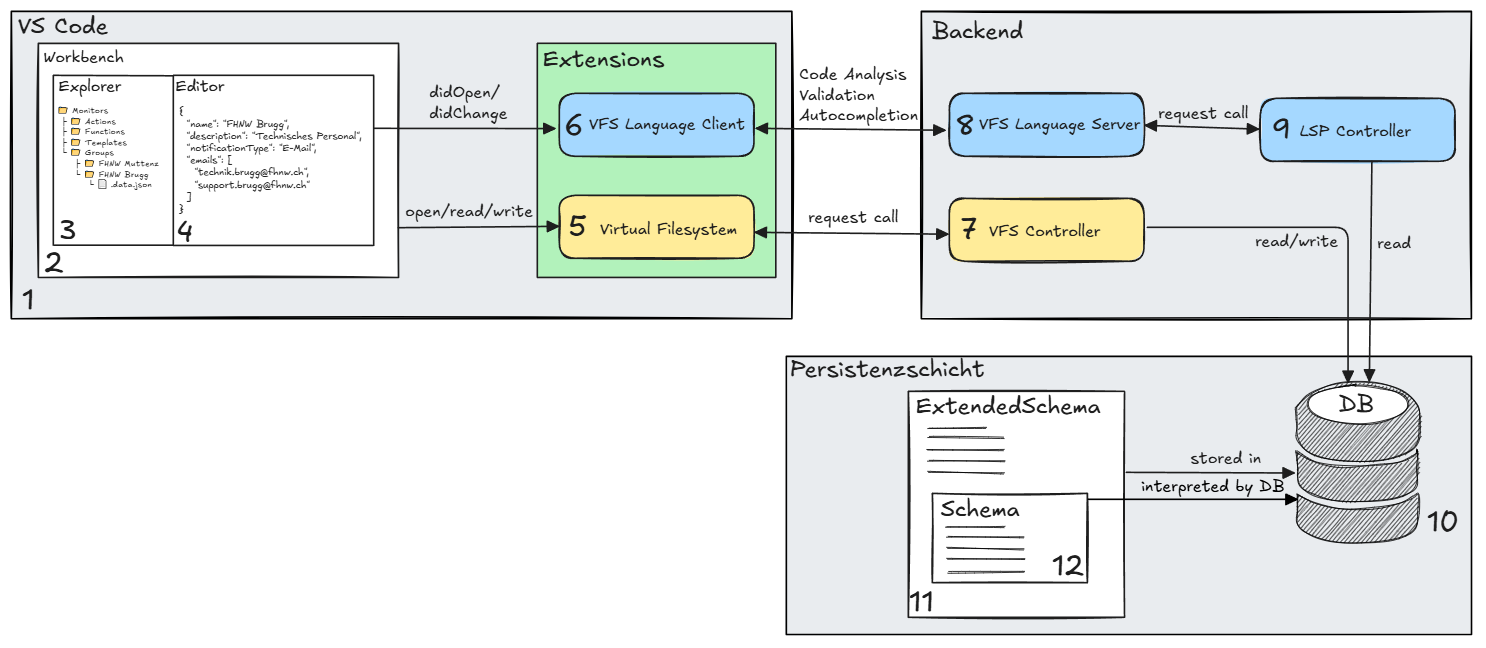
\includegraphics[width=1\linewidth]{arch.png}
    \caption{Architektur desMonidas Code Assist Navigator}
    \label{fig:architekturuebersicht}
\end{figure}

\section{Datenbankschema}
\label{kap:dbschema}
In diesem Kapitel werden die Anforderungen an das Datenbankschema beschrieben. Anschliessend wird ein vereinfachtes Domänenmodell vorgestellt, das als Grundlage für die weiteren Kapitel dient. Danach folgen die Beschreibung der Lösungsansätze und deren Umsetzung. Diese bildet die Grundlage für die Erläuterungen des Kapitel~\ref{kap:vfs} -~\ref{kap:lsp}.

\subsection{Anforderungen}
\label{abb:anforderungen}
Das Ziel dieser Bachelorarbeit ist die Entwicklung einer generischen, datenmodellgetriebenen Anwendung zur Verwaltung von IoT-Konfigurationen. Die Anwendungslogik soll dabei vollständig aus einem definierten Datenmodell abgeleitet werden, sodass Anpassungen im Quellcode vermieden werden. Daraus ergeben sich drei Anforderungen an das Datenbankschema: Erstens müssen Einstiegspunkte im Schema definiert werden, damit die Anwendung erkennt, wo der Verwaltungsprozess beginnt. Zweitens muss das Schema zusätzliche Validierungen unterstützen, da die verwendete Datenbanktechnologie Selva nur grundlegende Datentyp-Prüfungen bereitstellt. Drittens soll es möglich sein, zusätzliche Informationen wie beispielsweise Blattknoten oder potenzielle zyklische Verweise aus dem Schema abzuleiten, ohne dass diese im Schema definiert werden müssen.

\subsection{Domänenmodell}
\label{abb:domaenenmodell}
Das in Abschnitt~\ref{abb:tech} beschriebene Domänenmodell ist zu komplex, um es unverändert in der entwickelten Lösung zu verwenden. Deshalb wird zunächst ein vereinfachtes Modell definiert, das für die Umsetzung geeignet ist. Die Übertragbarkeit auf das Domänenmodell der Monidas-Plattform wird in Kapitel~\ref{kap:eva} untersucht.

Das für diese Arbeit verwendete Domänenmodell ist in Abbildung~\ref{ab:con} dargestellt und bildet ein typisches Szenario aus dem E-Commerce-Bereich ab. Das Modell besteht aus den fünf Entitäten: \textit{Customer}, \textit{Address}, \textit{Order}, \textit{LineItem} und \textit{Product}. Ein \textit{Customer} (Kunde) verfügt über Angaben wie Vorname, Nachname und eine E-Mail-Adresse. Jeder Kunde besitzt mehrere Adressen (\textit{Address}) und kann mehrere Bestellungen (\textit{Order}) tätigen. Eine Adresse umfasst die Strasse, Stadt sowie das Land und gehört eindeutig zu einem Kunden. Jede Bestellung besitzt eine Rechnungsadresse (\textit{billingAddress}) und optional eine Lieferadresse (\textit{shippingAddress}). Eine Bestellung besteht aus mindestens einer Bestellposition (\textit{LineItem}), welche jeweils ein Produkt (\textit{Product}) mit einer definierten Menge und einem Einzelpreis referenziert. Ein Produkt enthält eine eindeutige Beschreibung sowie einen Preis.

\begin{figure}[H]
    \centering
    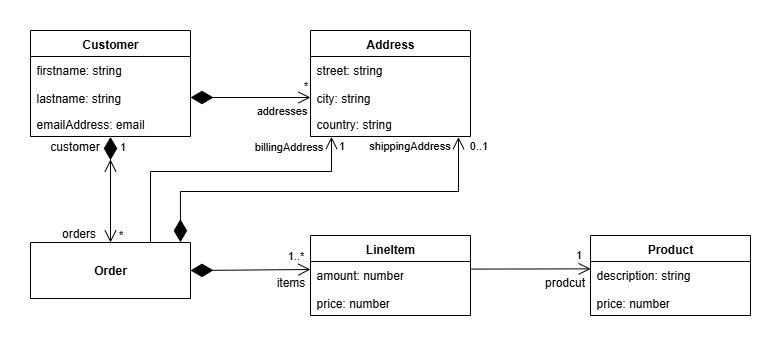
\includegraphics[width=0.8\linewidth]{Bsp_UML.png}
    \caption{Vereinfachtes Domänenmodell im E-Commerce-Kontext}
    \label{fig:uml_domaenenmodell}
\end{figure}

\subsection{Schemaerweiterungen}
Um die Anforderungen der Anwendung erfüllen zu können, mussten Erweiterungen am bestehenden Schema vorgenommen werden. Diese umfassen die Definition von Einstiegspunkten (Roots), Bedingungen (Constraints) sowie die dynamische Ableitung zusätzlicher Informationen.

\label{ab:con}
\subsubsection{Roots}
Unter dem Begriff «Roots» werden die im Schema definierten Einstiegspunkte verstanden. Diese bestimmen, bei welchen Entitäten die Navigation im virtuellen Filesystem beginnt. Für jeden Root wird ein Label festgelegt, das im Filesystem als Ordnername angezeigt wird. Dieses Label wird direkt im Schema definiert und kann unabhängig vom Namen der Entität frei gewählt werden.

Im E-Commerce-Domänenmodell (siehe Abbildung \ref{fig:uml_domaenenmodell}) könnten beispielsweise die Entitäten \textit{Customer} mit dem Label \textit{Customers} und \textit{Product} mit dem Label \textit{Products} als Roots definiert werden.

\subsubsection{Constraints}
Unter «Constraints» werden in dieser Thesis Bedingungen verstanden, die das Standardverhalten der Applikation gezielt ergänzen oder einschränken. Sie stellen sicher, dass die Daten bestimmte Anforderungen erfüllen und inhaltlich konsistent bleiben. Diese Bedingungen werden ausschliesslich von der Anwendungslogik geprüft und nicht von der Datenbank selbst.

Das Standardverhalten der Applikation sieht vor, dass neue Objekte direkt innerhalb ihres übergeordneten Knotens erstellt werden. Dieses Verhalten folgt einer Parent-Child-Hierarchie. Das Referenzieren eines bereits bestehenden Objekts ist standardmässig deaktiviert. Mit „Referenzieren“ wird in dieser Arbeit verstanden, dass beispielsweise bei einer Bestellung keine neue Adresse erstellt, sondern eine bereits existierende Adresse zugeordnet wird.

Werden jedoch zusätzliche Bedingungen benötigt, um das Standardverhalten gezielt zu erweitern, stehen die folgenden Constraints zur Verfügung: Pflichtfeld (notNull), bidirektionale Verknüpfung (bidirektional), Verbot der Erstellung neuer Objekte (denyCreation) und Erlaubnis zum Referenzieren bestehender Objekte (allowReference). Zur Veranschaulichung dieser Constraints dient folgendes Beispiel aus dem E-Commerce-Domänenmodell:

Beim Erstellen eines neuen Kunden ist die Angabe einer E-Mail-Adresse zwingend erforderlich (notNull), andernfalls ist das Speichern nicht möglich. Anschliessend erstellt der Kunde zwei Adressen, beispielsweise eine Heimadresse und eine Arbeitsadresse, welche eindeutig diesem Kunden zugeordnet sind. Möchte der Kunde eine Bestellung tätigen, ist dafür zwingend die Angabe einer Rechnungsadresse (billingAddress) erforderlich (notNull). Innerhalb der Bestellung ist das Erstellen einer neuen Rechnungsadresse technisch nicht möglich, da dies explizit deaktiviert wurde (denyCreation). Stattdessen muss eine bereits vorhandene Adresse ausgewählt werden (allowReference), beispielsweise die zuvor erstellte Arbeitsadresse. Darüber hinaus muss jede Bestellung mindestens eine Bestellposition enthalten (notNull). Diese Bestellposition wird direkt im Kontext der Bestellung erstellt und muss zwingend auf ein bereits bestehendes Produkt (Product) verweisen (allowReference, denyCreation). Optional kann zudem eine Lieferadresse angegeben werden. Diese Lieferadresse wird direkt im Kontext der Bestellung erstellt und existiert ausschliesslich dort. Das Referenzieren bereits bestehender Adressen, beispielsweise der Heim- oder Arbeitsadresse, ist hierbei technisch deaktiviert und daher nicht möglich (Standardverhalten).

\subsubsection{Schema Analyse}
\label{sec:dynamischerAb}
Die zuvor beschriebenen Schemaerweiterungen wie Constraints und Roots werden statisch definiert. Eine weitere Information, nämlich ob ein Referenzfeld zu einem Blattknoten (\textit{isLeaf}) führt, lässt sich hingegen durch eine Schema-Analyse ableiten. Ein Blattknoten bezeichnet hierbei einen Knoten, dessen Entitätstyp keine weiteren ausgehenden Referenzen besitzt. Diese ermittelte Information wird genutzt, um Darstellungs- und Bearbeitungslogiken innerhalb des virtuellen Filesystems zu steuern. Die konkrete Verwendung wird detailliert in Kapitel~\ref{kap:vfs} erläutert. Dies wird direkt im Schema ergänzt, wodurch sich der Modellierungsaufwand reduziert und die Flexibilität für Erweiterungen steigt.

Für die Schema-Analyse wird das Schema als gerichteter Graph interpretiert. Entitätstypen wie \textit{Customer}, \textit{Order}, \textit{Address}, \textit{LineItem} und \textit{Product} bilden dabei die Knoten, während Referenzfelder wie \textit{addresses}, \textit{billingAddress}, \textit{shippingAddress}, \textit{customer}, \textit{items} und \textit{product} die gerichteten Kanten darstellen. Zur Traversierung des Graphen wird der Algorithmus der Tiefensuche (Depth-First Search, DFS) verwendet. Dabei handelt es sich um einen Graphen-Algorithmus, der von einem Startknoten ausgehend zunächst einen Pfad vollständig verfolgt, bevor zurückgegangen und der nächste Pfad untersucht wird. 

\begin{figure}[H]
    \centering
    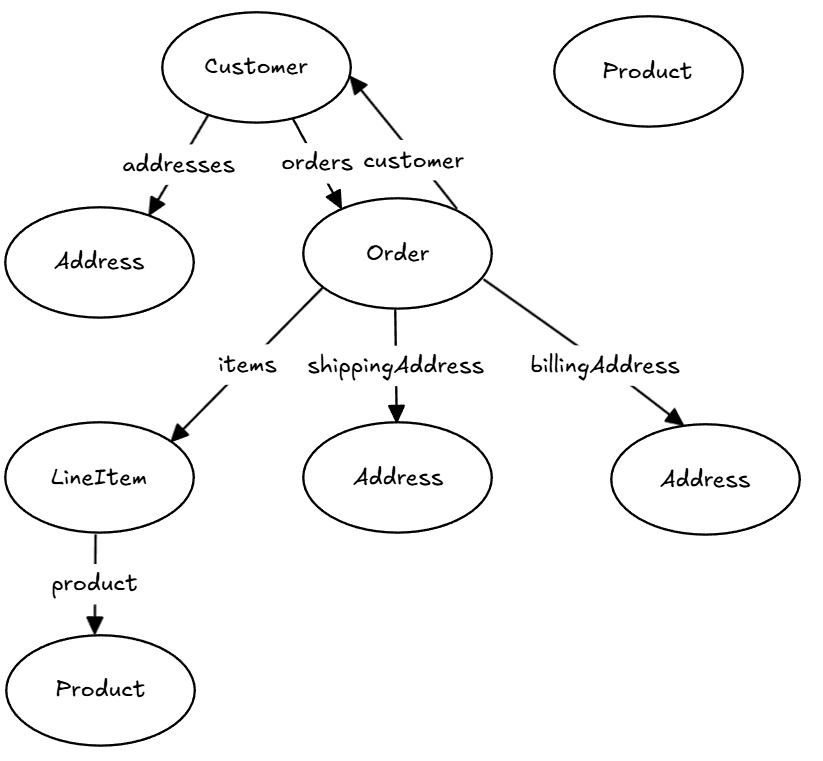
\includegraphics[width=0.8\linewidth]{dag.png}
    \caption{Gerichtete Graphdarstellung des E-Commerce-Datenbankschemas}
    \label{fig:dag}
\end{figure}
\newpage

Im Rahmen der Lösungsfindung wurden weitere Ansätze zur Informationsableitung geprüft. Einer dieser Ansätze bestand darin, sämtliche möglichen URIs bereits im Vorfeld aus dem Schema abzuleiten. Ein URI (Uniform Resource Identifier) bezeichnet hierbei einen eindeutigen Pfad, der sich aus der Abfolge von Referenzfeldern (gerichteten Kanten) und Instanzen von Entitätstypen (Knoten) zusammensetzt. Eine Instanz bezeichnet dabei ein konkretes Datenobjekt, das auf Basis einer im Schema definierten Entität erzeugt wurde. Beispielsweise ergibt sich ein URI aus einer Abfolge wie:

\begin{center}
\texttt{Customers/\{customerId\}/Orders/\{orderId\}}
\end{center}

Ziel dieses Ansatzes war es, alle gültigen URI-Muster im Vorfeld zu ermitteln, um URIs zur Laufzeit validieren zu können. Dieses Vorgehen ist allerdings nur geeignet, wenn im Schema keine Zyklen auftreten. Sobald zyklische Referenzen vorhanden sind, entstehen theoretisch unendlich viele URI-Kombinationen. Daher lässt sich dieser Ansatz bei zyklischen Schemata nicht allgemein anwenden.

Ein weiterer untersuchter Ansatz bestand darin, die genaue Pfadtiefe eines URI bereits im Voraus zu ermitteln. Da jedoch eine vollständige Abbildung aller möglichen URIs vorab nicht realisierbar war und sich die Pfadtiefe ohnehin einfach direkt aus dem URI während einer Anfrage ableiten lässt, erwies sich dieser Ansatz letztlich als nicht zielführend und wurde verworfen.
%hasPossbileCycle
%\subsection{Bereitstellung und Zugriff}

\subsection{Umsetzung}

\subsubsection{Roots und Constraints}
Die Definition von Einstiegspunkten („Roots“) sowie zusätzlichen Validierungen („Constraints“) erfordert eine Erweiterung der ursprünglichen TypeScript-Typdefinition aus der Colombalink-Bibliothek. Für die Umsetzung wurde das bestehende Schema aus der Colombalink-Bibliothek angepasst. Dabei wurde die Typdefintion Schema erweitert, um die Definition von Roots und Constraints zu ermöglichen. Die dafür notwendigen TypeScript-Features wie Omit, Intersection Types, Union Types und Generics stellten sicher, dass diese Erweiterung umgesetzt werden konnte~\cite{typescript:handbook}. Das Ergebnis ist ein erweitertes Schema, das den Anforderungen aus Abschnitt~\ref{abb:anforderungen} entspricht. Die genaue technische Umsetzung befindet sich im Anhang in Listing~\ref{lst:extended-schema}.

Im vorherigen Abschnitt wurde bereits erläutert, wie im konkreten E-Commerce-Domänen\-modell die Entitäten \textit{Customer} und \textit{Product} als Roots definiert wurden, sowie welche Constraints für die Entität \textit{Order} gesetzt wurden. Im nachfolgenden Listing~\ref{lst:con} ist dargestellt, wie dies im erweiterten Schema definiert werden können.

\newpage
\lstinputlisting[
caption={Definition von Roots und Constraints im erweiterten Schema},
label={lst:con},
style=customtypescript
]{listings/con.json}

\newpage
\subsubsection{Schema Analyse}
Die technische Umsetzung der Schema-Analyse erfolgt mithilfe einer rekursiven Tiefensuche. Ausgangspunkte der Traversierung sind die zuvor definierten Einstiegspunkte (\textit{Customer} und \textit{Product}, siehe Abschnitt~\ref{ab:con}).

Während der Tiefensuche wird jeder besuchte Entitätstyp (Knoten) erfasst. Wird ein bereits besuchter Knoten erneut erreicht, deutet dies auf einen möglichen Zyklus hin und die weitere Traversierung entlang dieses Pfades wird beendet. Hat ein referenzierter Knoten keine weiteren ausgehenden Referenzen, wird das Feld \texttt{isLeaf} gesetzt, um ihn als Blattknoten zu kennzeichnen.

Das Ergebnis der Schema-Analyse für das E-Commerce-Schema ist in Tabelle~\ref{tab:schema-analyse-dfs} dargestellt. Der zugehörige Code befindet sich im Anhang (Listing~\ref{lst:extendSchemaDFS}).

\begin{table}[H]
  \centering
  \begin{tabular}{lllc}
    \toprule
    \textbf{Ausgangsknoten} & \textbf{Referenz (Kante)} & \textbf{Zielknoten} & \textbf{isLeaf}\\ 
    \midrule
    Product & – & – & – \\[4pt]
    Customer & addresses & Address & Ja \\[4pt]
    Customer & orders & Order & Nein \\[4pt]
    Order & billingAddress & Address & Ja \\[4pt]
    Order & shippingAddress & Address & Ja \\[4pt]
    Order & items & LineItem & Nein \\[4pt]
    LineItem & product & Product & Ja \\[4pt]
    Order & customer & Customer & Nein \\ 
    \bottomrule
  \end{tabular}
  \caption{Ergebnis der Schema-Analyse mit DFS für das E-Commerce-Schema}
  \label{tab:schema-analyse-dfs}
\end{table}



\section{Virtuelles Filesystem}
\label{kap:vfs}
Dieses Kapitel beschreibt die Umsetzung des virtuellen Filesystems (VFS). Ziel der Umsetzung ist es, die in Kapitel~\ref{sec:problemstellung} beschriebenen Herausforderungen zu lösen. Im Folgenden werden zunächst die konzeptionellen Überlegungen vorgestellt, bevor auf die technische Umsetzung eingegangen wird.

\subsection{Lösungsansätze}
\label{sec:vfs-konzeption}
In diesem Abschnitt werden verschiedene Lösungsansätze zur Umsetzung des VFS vorgestellt und bewertet. Die Komponenten „Explorer“ und „Editor“ werden getrennt betrachtet, da ihre Aufgaben unterschiedlich sind. Zum Schluss folgt eine gemeinsame Betrachtung beider Komponenten.

\subsubsection{Explorer}
Wie bereits in Kapitel~\ref{kap:Architek} beschrieben, dient der Explorer der Navigation durch die Instanzen. Grundlage hierfür bildet das Datenbankschema. Vor der Umsetzung sind folgende konzeptionelle Fragen zu klären:
\begin{itemize}
  \item Wie wird die URI-Struktur generiert?
    \item Wie ist die Benutzeroberfläche gestaltet?
    \item Wie werden die Daten bereitgestellt?
    \item Wie werden Referenzen, Zyklen und Blattknoten beim Traversieren behandelt?
    \item Welche Funktionen bietet der Explorer und welche Einschränkungen bestehen?
\end{itemize}

\subsubsection*{URI Konzept}
\label{sec:urikonzept}
Eine Uniform Resource Identifier ist eine Zeichenfolge zur eindeutigen Identifikation und zur Beschreibung der hierarchischen Position einer Ressource. Aus einer URI lassen sich die Position einer Ressource innerhalb der Struktur sowie deren Beziehungen zu anderen Ressourcen ableiten~\cite{rfc3986}.

In dieser Arbeit werden URIs verwendet, um Instanzen eindeutig zu identifizieren, deren Beziehungen zueinander zu erkennen und sie in einer Baumstruktur im Filesystem abzubilden. Die Struktur einer URI ergibt sich, wie bereits in Abschnitt~\ref{sec:dynamischerAb} beschrieben, aus der Kombination des Namens eines Referenzfeldes und eines eindeutigen Bezeichners der Instanz. Damit jede Instanz innerhalb dieser Struktur eindeutig und zugleich verständlich benannt werden kann, wird das bisher vorgestellte Domänenmodell (siehe Kapitel~\ref{kap:dbschema}) um ein neues Feld erweitert: den „Slug“. Ein Slug ist eine eindeutige Bezeichnung vom Typ \texttt{string}, die für jede Instanz im Datenbankschema definiert werden muss. Der Slug wird beim Erstellen einer neuen Instanz im Explorer vergeben und entspricht dabei dem Namen des Ordners.

Die URI folgt einem festen Muster: Ungerade Segmente enthalten den Namen des Referenzfeldes aus dem Datenmodell, wobei der erste Buchstabe grossgeschrieben wird (z.B. wird aus „addressen“ immer „Addressen“). Gerade Segmente enthalten den Slug der zugehörigen Instanz. Einstiegspunkte (Roots) besitzen kein Referenzfeld, weshalb hier das im Schema definierte Label als erstes URI-Segment verwendet wird. Jeder Slug muss innerhalb seines Pfades eindeutig sein. Diese Eindeutigkeit stellt der Explorer beim Erstellen neuer Instanzen sicher und wird zusätzlich durch den VFS-Controller geprüft.

Ein Beispiel verdeutlicht diesen Aufbau: Erstellt ein Systemintegrator einen neuen Kunden mit dem Ordnernamen „max“, so ergibt sich die URI \texttt{/Customers/max}. Dabei ist „Customers“ das Label des Root-Typs, und „max“ der eindeutig vergebene Slug der Instanz.


%Gehört in Umsetzung
%Wie in Abschnitt~\ref{sec:Datenzugriff} beschrieben, wird die URI beim Erstellen einer Instanz als Alias in der Selva-Datenbank gespeichert. Dafür wird die entsprechende Alias-Funktion der Datenbank genutzt. Dadurch ist jede Instanz direkt über ihre URI abrufbar. Aus dem URI-Verlauf lassen sich zudem abhängige Kindinstanzen ableiten. Die URI-Struktur reduziert somit die Komplexität bei der Datenbereitstellung im virtuellen Filesystem und vereinfacht die Implementierung des Language Servers.


%Jede URI ist eindeutig und wird als Referenzpfad verwendet. In der Datenbank dient sie gleichzeitig als Alias, um eine  Identifikation und Navigation zu ermöglichen (siehe Abschnitt~\ref{sec:Datenzugriff}).

%Zudem bildet das URI-Konzept die Grundlage für die Implementierung des Language Servers (siehe Kapitel~\ref{sec:lsp}). Der Language Server kennt ausschliesslich die URI sowie den Inhalt der aktuell im Editor geöffneten Datei. Da jede Instanz eindeutig über ihre URI identifiziert wird, reduziert sich die Komplexität bei der Implementierung des Language Servers deutlich. Zusätzliche interne Identifikatoren müssen im Editor nicht verwaltet werden.

\subsubsection*{Benutzeroberfläche}
\label{par:uiExploerer}
Die Benutzeroberfläche basiert auf der integrierten Explorer-Ansicht von Visual Studio Code. Der Explorer stellt grundlegende Dateioperationen wie das Erstellen, Umbenennen, Löschen und Verschieben von Dateien und Ordnern zur Verfügung und ermöglicht die Navigation innerhalb der Verzeichnisstruktur. Da diese Aktionen systemseitig nicht deaktiviert werden können, ergeben sich Einschränkungen bei bestimmten Nutzeraktionen. Diese werden im Abschnitt~\ref{sec:Nutzeraktionen} näher erläutert. Eine zusätzliche technische Begrenzung besteht darin, dass die Editor-Komponente nicht um weitere Bedienelemente, wie beispielsweise Schaltflächen, erweitert werden kann. Individuelle Icons innerhalb der Explorer-Ansicht wären technisch umsetzbar, wurden jedoch im Rahmen dieser Arbeit nicht implementiert.

Zur Verdeutlichung wird die Darstellung des Explorers anhand des zuvor eingeführten Domänenmodells (siehe Abschnitt~\ref{kap:dbschema}) in Abbildung~\ref{fig:explorer-ui} gezeigt.

\begin{figure}[H]
  \centering
  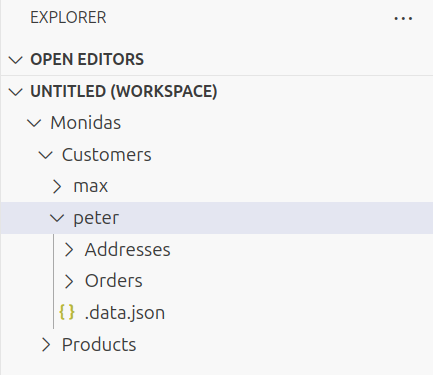
\includegraphics[width=0.4\linewidth]{explorer-ui.png}
  \caption{}
  \label{fig:explorer-ui}
\end{figure}

Wie aus der Abbildung ersichtlich, entspricht die Struktur des Explorers dem zuvor eingeführten URI-Konzept (siehe Abschnitt~\ref{sec:vfs-konzeption}). Auf oberster Ebene befinden sich die bekannten Root-Ordner. Darunter folgen Ordner für einzelne Instanzen. Beim Öffnen einer Instanz wird eine Datei mit dem Namen \texttt{.data.json} angezeigt, welche die Instanzdaten im JSON-Format enthält. Zusätzlich erscheinen Ordner, deren Bezeichnungen sich unmittelbar aus den Referenzfeldern des Datenbankschemas ableiten. Die genaue Bedeutung und Nutzung der Datei wird in Abschnitt~\ref{sec:Editor} erläutert.

Beim Aufklappen der Ordner ergeben sich spezielle Darstellungs- und Navigationsfälle, welche gesondert evaluiert wurden. Diese werden in Abschnitt~\ref{sec:referenz-zyklusbehandlung} und Abschnitt~\ref{sec:blattknoten} erläutert.

Für eine einheitliche Darstellung im weiteren Verlauf der Arbeit werden die Begriffe «Root-Ordner» für oberste Einstiegspunkte, «Referenzordner» für aus Referenzfeldern abgeleitete Ordner und «Instanzordner» für Ordner der Instanzen verwendet.

\newpage
\subsubsection*{Bereitstellung der Daten}
Die Bereitstellung der Daten beschreibt, wie die im Explorer benötigten Daten technisch geladen und dargestellt werden. Nutzeraktionen, beispielsweise das Öffnen oder Aufklappen eines Ordners im Explorer, lösen Datenanfragen durch die VFS-Extension aus. Für diese Datenbereitstellung wurden zwei Lösungsansätze untersucht: das Pull-Prinzip und das Push-Prinzip.

Beim Pull-Prinzip fordert die VFS-Extension die Daten erst dann vom VFS-Controller an, wenn eine entsprechende Nutzeraktion erfolgt. Ein wesentlicher Vorteil hierbei ist, dass tatsächlich benötigte Daten geladen werden und der Datenaustausch klar steuerbar bleibt. Ein Nachteil liegt allerdings darin, dass externe Datenänderungen, wie etwa Änderungen durch andere Nutzer oder Prozesse im Hintergrund, nicht erkannt werden, da Daten nur auf Anfrage hin aktualisiert werden.

Alternativ wurde das Push-Prinzip untersucht. Bei diesem Ansatz werden Datenänderungen vom Controller proaktiv an die VFS-Extension gesendet. Dabei abonniert die VFS-Extension Benachrichtigungskanäle, die sie über Datenänderungen informieren. Jedoch zeigten sich bei diesem Ansatz Schwierigkeiten, da interne Aktionen wie das erneute Rendern sämtlicher geöffneter Ordner im Explorer komplexe Logiken zur Verwaltung der Subscriptions erfordern. Dies führte zu erhöhtem Aufwand und Implementierungsschwierigkeiten.

Aufgrund der geringeren Komplexität, besseren Steuerbarkeit und bewussten Nichtberücksichtigung von Multi-User-Szenarien wurde das Pull-Prinzip gewählt. Zukünftige Erweiterungen könnten dieses Prinzip bei Bedarf ergänzen, indem wichtige externe Änderungen über gezielte, eventbasierte Push-Benachrichtigungen übertragen werden. Technische Einzelheiten zur Umsetzung sind im Abschnitt \ref{subsec:explorer-baum} beschrieben.


\subsubsection*{Referenz- und Zyklusbehandlung}
\label{sec:referenz-zyklusbehandlung}
Beim Navigieren im Explorer können Instanzen andere Instanzen referenzieren. Dadurch stellt sich die konzeptionelle Frage, wie der Explorer beim Aufklappen von Ordnern mit solchen Referenzen umgehen soll. Ein Sonderfall entsteht, wenn dieselbe Instanz innerhalb eines Pfades erneut vorkommt. Man spricht dann von einem \textit{Zyklus}. 

Für die Behandlung dieser Situationen wurden zwei Lösungsansätze geprüft:

Beim ersten Ansatz werden zyklische Referenzen vollständig aufgeklappt dargestellt, wodurch dieselbe Instanz mehrfach im Explorer erscheint. Der Vorteil dieses Ansatzes besteht in einer flexiblen und uneingeschränkten Navigation für den Benutzer. Während der Evaluierung zeigte sich allerdings, dass die technische Komplexität der VFS-Extension dadurch erheblich zunimmt. Zwar ermöglichen interne IDs eine eindeutige Identifikation der Instanzen, zusätzlich wäre jedoch ein Mechanismus für symbolische Verknüpfungen („Softlinks“) erforderlich. Dieser würde sicherstellen, dass Änderungen an einer Instanz konsistent auf alle mehrfach dargestellten Kopien übertragen werden.

Der zweite Lösungsansatz verhindert von vornherein das Aufklappen referenzierter Instanzen im Explorer. Sobald eine bestehende Instanz erneut referenziert wird, lässt die Anwendung kein weiteres Aufklappen zu, wodurch Zyklen grundsätzlich vermieden werden. Ein wesentlicher Vorteil ist die deutlich geringere technische Komplexität, da Mehrfachdarstellungen und deren Synchronisation vollständig entfallen. Die dadurch entstehende Einschränkung in der Navigation wird durch eine ergänzende „Jump-to-Definition“-Funktion kompensiert, die Nutzern das direkte Navigieren zur ursprünglichen Instanz ermöglicht. Die Umsetzung dieser Funktion wird im Abschnitt zum Language Server ausführlich erläutert.

\subsubsection*{Blattknoten}
\label{sec:blattknoten}
Im Rahmen der konzeptionellen Darstellung im Explorer stellt sich die Frage, wie Instanzen dargestellt werden sollen, die laut Datenbankschema nur einmal pro übergeordnetem Objekt erstellt werden können. Im aktuellen Domänenmodell wurde beispielsweise festgelegt, dass ein Kunde mehrere Adressen erstellen darf. Falls jedoch das Schema so definiert wäre, dass ein Kunde nur exakt eine Adresse erstellen kann, ergibt sich die Frage, wie diese einzelne Instanz im Explorer dargestellt werden soll. \footnote{Die Abbildungen~\ref{fig:noinline} und~\ref{fig:inline} sind hypothetischen und entsprechen nicht dem Domänenmodell aus Abschnitt \ref{abb:domaenenmodell}.}


Dafür wurden zwei mögliche Lösungsansätze betrachtet:

\textbf{Reguläre Darstellung}\\
Blattknoten werden analog zu regulären Instanzen als separate, aufklappbare Ordner dargestellt. Dies hätte den Vorteil, dass keine zusätzliche technische Logik notwendig wäre, um Blattknoten speziell zu erkennen. Als Nachteil entsteht jedoch eine erhöhte Navigationskomplexität, da zusätzliche Hierarchieebenen entstehen.

\textbf{Inline-Darstellung}\\
Blattknoten werden direkt innerhalb der Parent-Instanz dargestellt, wodurch eine zusätzliche Navigationsebene entfällt. Diese Variante verbessert die Übersichtlichkeit deutlich. Nachteilig ist allerdings der erhöhte Implementierungsaufwand, da Blattknoten explizit erkannt und gesondert behandelt werden müssen. Zudem ist für Nutzer erst nach dem Öffnen der Parent-Instanz ersichtlich, ob ein Blattknoten überhaupt existiert.

\begin{figure}[H]
    \centering
      \begin{minipage}{0.45\textwidth}
        \centering
        \includegraphics[width=1\linewidth]{noinline.png}
        \caption{Reguläre Darstellung}
        \label{fig:noinline}
    \end{minipage}\hfill
    \begin{minipage}{0.45\textwidth}
        \centering
        \includegraphics[width=1\linewidth]{inline.png}
        \caption{Inline-Darstellung}
        \label{fig:inline}
    \end{minipage}
\end{figure}

Aufgrund der verbesserten Übersichtlichkeit und der Reduktion unnötiger Navigationsschritte wurde trotz des höheren Implementierungsaufwands die Inline-Darstellung innerhalb der Datei gewählt. Für eine mögliche Erweiterung der Anwendung wäre es denkbar, dem Nutzer die Wahl der bevorzugten Darstellung zu überlassen, beispielsweise über eine entsprechende Einstellung in der Benutzeroberfläche.

\newpage
\subsubsection*{Nutzeraktionen im Explorer}
\label{sec:Nutzeraktionen}
Wie in Abschnitt~\ref{par:uiExploerer} beschrieben, stehen im Explorer die Standardaktionen eines Filesystems zur Verfügung. Da die Struktur des Explorers direkt durch das zugrunde liegende Datenbankschema bestimmt wird, sind einzelne Aktionen gezielt eingeschränkt. Im Folgenden wird erläutert, wie diese Aktionen durchgeführt werden, auf welche Ordner und Dateien sie angewendet werden können und weshalb dabei bestimmte Einschränkungen erforderlich sind.

\textbf{Ordner erstellen}\\
Mit dem Erstellen eines neuen Ordners leitet man im Monidas CAN den Erstellprozess einer neuen Instanz ein. Wie ein Erstellprozess definiert ist, wird im Abschnitt~\ref{sec:Editor} beschrieben, da dieser Abhängigkeiten zum Editor aufweist. Aus diesem Grund ist das Erstellen nur auf Ebene der Root- und Referenzordner möglich. Auf Instanzordner-Ebene ist das Erstellen dagegen nicht erlaubt, da jede Instanz zwingend auf einer definierten Entität im Datenbankschema basieren muss. Versuche, auf Instanzordner-Ebene einen Ordner zu erstellen, werden mit einer Popup-Fehlermeldung abgelehnt.

\textbf{Datei erstellen}\\
Das Erstellen einer Datei ist auf keiner Ordnerebene erlaubt. Die einzige erlaubte Datei ist die von der VFS-Extension bereitgestellte data.json. Diese Datei stellt die Daten einer Instanz zur Bearbeitung im Editor bereit. Da das virtuelle Filesystem keine lokalen Dateien speichert, werden Instanzdaten erst beim Zugriff aus der Datenbank geladen. Zusätzliche Dateien hätten keinen Bezug zum definierten Datenbankschema und könnten somit nicht von der Anwendung verarbeitet oder verwaltet werden. Solche Dateien wären wirkungslos für die Datenverwaltung und daher unnötig. Aus diesem Grund werden Versuche, weitere Dateien zu erstellen, abgelehnt. Dem Benutzer wird eine Popup-Fehlermeldung angezeigt.

\textbf{Umbenennen}\\
Nur Instanzordner dürfen umbenannt werden. Root- und Referenzordner haben feste Namen aus dem Datenbankschema und dürfen daher nicht geändert werden. Auch die Datei data.json darf nicht umbenannt werden, da sie als eindeutiger Zugriffspunkt auf die Instanzdaten dient. Ein Umbenennen würde den Datenzugriff verhindern. Unzulässige Umbenennungen werden mit einer Popup-Fehlermeldung abgelehnt.

%Beim Umbenennen eines Instanzordners verändert sich der Slug und somit auch die eindeutige URI der Instanz. Dabei wird das Feld aliases, welches die URI speichert, angepasst und alle abhängigen URIs aktualisiert. „Abhängige URIs“ sind URIs von Instanzen, die auf die umbenannte Instanz verweisen.

\textbf{Löschen}\\
Ein Löschvorgang ist, analog zur Umbenennung, nur auf Instanzordnern zulässig. Root- und Referenzordner sowie die Datei \texttt{data.json} sind dagegen fest vorgegeben und dürfen nicht gelöscht werden. Aufgrund der Integration in das VS-Code-Filesystem erscheint bei jedem Löschversuch ein Bestätigungsdialog, welcher sich nicht deaktivieren lässt. Daraus entsteht der Nachteil, dass selbst bei unzulässigen Löschaktionen zuerst der Bestätigungsdialog bestätigt werden muss. Erst danach folgt die eigentliche Fehlermeldung, die ebenfalls als Dialog und nicht als einfache Popup-Meldung dargestellt werden kann.

Anzumerken ist auch, dass in dieser Arbeit keine Löschregeln (Delete-Policies) berücksichtigt wurden. Solche Regeln bestimmen, ob ein Objekt gelöscht werden darf, wenn andere Objekte darauf verweisen. Selva unterstützt diese Funktionalität nicht. Colomba Link bietet zwar eine eigene Datenbank-Implementierung, doch diese ist derzeit nicht URI-kompatibel. Da Colomba Link plant, diese Erweiterung selbst vorzunehmen, wurde bewusst auf eine eigene Umsetzung verzichtet.

\subsubsection*{Verschieben}
Das Verschieben von Ordnern und Dateien wird auf keiner Ordnerebene unterstützt. Theoretisch möglich wäre das Verschieben eines Instanzordners zwischen Referenzordnern desselben Entitätstyps. Ein Beispiel hierfür wäre das Verschieben der Heimadresse des Kunden \texttt{max} in den Adressordner des Kunden \texttt{peter}:

\begin{verbatim}
/Customers/max/Addresses/homeAddress → /Customers/peter/Addresses/
\end{verbatim}

Eine Voraussetzung hierfür wäre, dass keine anderen Instanzen auf die verschobene Instanz verweisen. Die Implementierung einer solchen Prüfung ist komplex und konnte im Rahmen dieser Arbeit zeitlich nicht berücksichtigt werden. Aus diesem Grund wird das Verschieben generell verhindert und jeder Versuch mit einer Fehlermeldung abgelehnt. Dasselbe gilt analog auch für die Aktion „Kopieren“.


\subsubsection{Editor}
\label{sec:Editor}
Während der Explorer die Navigation durch Instanzen ermöglicht, dient der Editor der Erstellung und Bearbeitung dieser Instanzen. Vor der Umsetzung sind folgende konzeptionelle Fragen zu klären:

\begin{itemize}
\item Warum erfolgt die Bearbeitung der Instanzdaten über eine (\texttt{.data.json}) Datei?
\item Wie werden Instanzen im Editor dargestellt?
\item Wie beeinflusst die Inline-Darstellung im Explorer das Bearbeitungskonzept im Editor?
\item Welche Validierungen sind erforderlich?
\item Welche Aufgaben übernimmt der Editor nicht?
\end{itemize}

\subsubsection*{Dateiformat}
Die Entscheidung, Instanzdaten pro Instanz in genau einer Datei im JSON-Format (.data.json) bereitzustellen, basiert auf konzeptionellen und technischen Gründen. Die Verwendung genau einer Datei pro Instanz reduziert die Komplexität bei der Navigation sowie der Bearbeitung der Instanzen, da sämtliche Daten an einer Stelle zusammengefasst sind. Dies verhindert, dass Nutzende während der Bearbeitung zwischen mehreren Dateien wechseln müssen.

Das JSON-Format wurde gewählt, weil es strukturierte Daten übersichtlich darstellt und von Menschen sowie Maschinen einfach verarbeitet werden kann. Aufgrund seiner weiten Verbreitung und Standardisierung eignet es sich besonders für den Datenaustausch zwischen den Komponenten der Anwendung.

Ein weiterer Grund für die Wahl des JSON-Formats ist dessen bisherige Verwendung innerhalb der Monidas-Plattform. Bereits bestehende Komponenten der Plattform nutzen JSON zur Verwaltung und Konfiguration von Sensor- und Monitorparametern (siehe Abschnitt \ref{kap:konf}). Diese Konsistenz vereinfacht die Integration und Wartbarkeit der Lösung.

Technisch ermöglicht JSON eine direkte Bearbeitung im Editor von Visual Studio Code ohne zusätzlichen Implementierungsaufwand. Zudem stellt JSON die Grundlage für Editorfunktionen wie Validierung und Autovervollständigung dar, die über den Language Server umgesetzt werden (siehe Kapitel \ref{kap:lsp}).

\newpage
\subsubsection*{Benutzeroberfläche}
Die Benutzeroberfläche zur Bearbeitung der Instanzdaten basiert auf der integrierten Editor-Komponente von Visual Studio Code. Beim Öffnen der Datei .data.json werden sämtliche Felder einer Instanz angezeigt. Diese Felder entsprechen direkt den im Datenbankschema definierten Feldern und werden im Editor stets nach einer festgelegten Reihenfolge dargestellt, um eine konsistente Bearbeitung zu gewährleisten.

Das Feld slug, welches als Ordnername einer Instanz im Explorer verwendet wird, ist im Editor nicht sichtbar. Änderungen am slug erfolgen über die Umbenennungsfunktion des Explorers (siehe Abschnitt~\ref{sec:Nutzeraktionen}). Diese bewusste Trennung vermeidet zusätzlichen Aufwand, welcher durch notwendige Validierungen und Synchronisationsprozesse zwischen Explorer und Editor entstehen würde.

Die im Editor dargestellten Felder entsprechen den im Datenbankschema definierten Datentypen (siehe Abschnitt \ref{sec:Datenzugriff}). Einfache Datentypen (string, boolean, number) werden als entsprechende JSON-Werte dargestellt. Referenzfelder (reference, references) werden grundsätzlich mit einer Kombination aus eindeutiger ID und dem slug der referenzierten Instanz angezeigt. Diese Darstellung dient als Hinweis auf die Herkunft der referenzierten Instanz und unterstützt die spätere Editorfunktionalität des Language Servers, zur Navigation („Jump-to-Definition“). Weiterführende Informationen zur Darstellung und den unterstützenden Editorfunktionen werden im Kapitel zur Editorunterstützung mit LSP detailliert beschrieben (siehe Kapitel \ref{kap:lsp}).

Eine Ausnahme zur oben beschriebenen Darstellung bilden Blattknoten, deren Darstellung und Erstellung im Editor im folgenden Abschnitt näher erläutert werden (siehe Abschnitt \ref{sec:EDblattknoten}).

\begin{figure}[H]
\centering
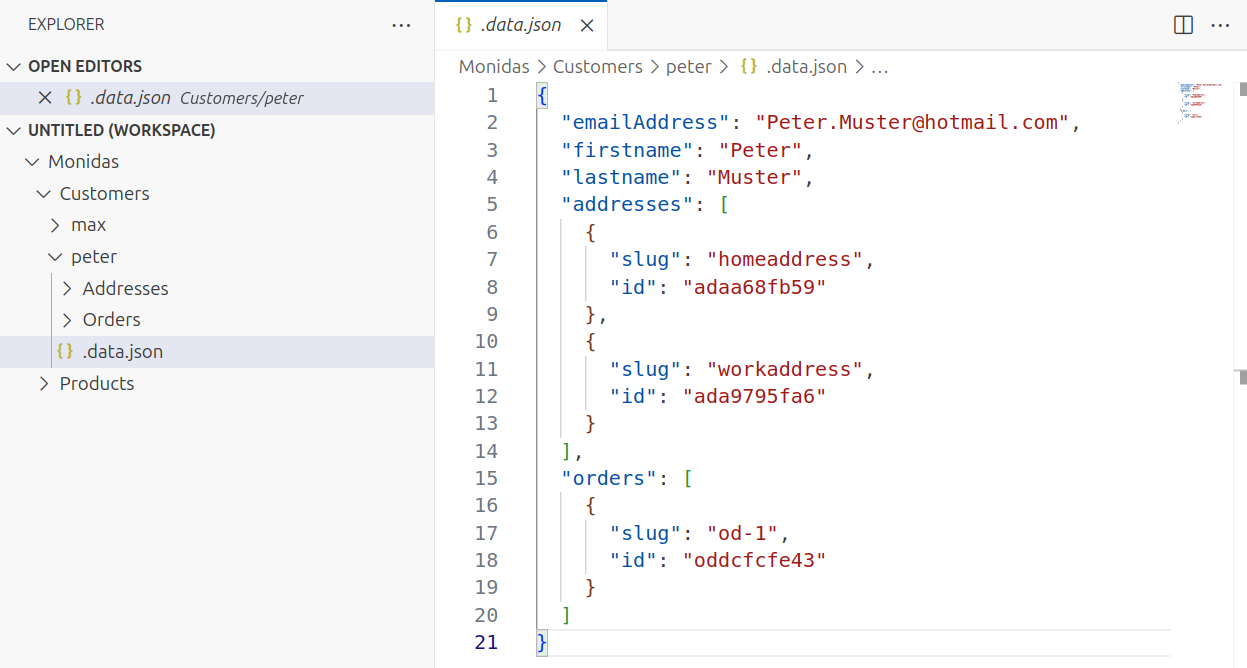
\includegraphics[width=0.9\linewidth]{editor-ui.png}
\caption{Darstellung der Instanzdaten im Editor}
\label{fig:editor-ui}
\end{figure}

\newpage
\subsubsection*{Blattknoten}
\label{sec:EDblattknoten}
Wie bereits in Abschnitt \ref{sec:blattknoten} beschrieben, weicht die Darstellung und Bearbeitung von Blattknoten im Editor von der Standarddarstellung ab. Im Folgenden werden diese Unterschiede detailliert erläutert.

\begin{figure}[H]
\centering
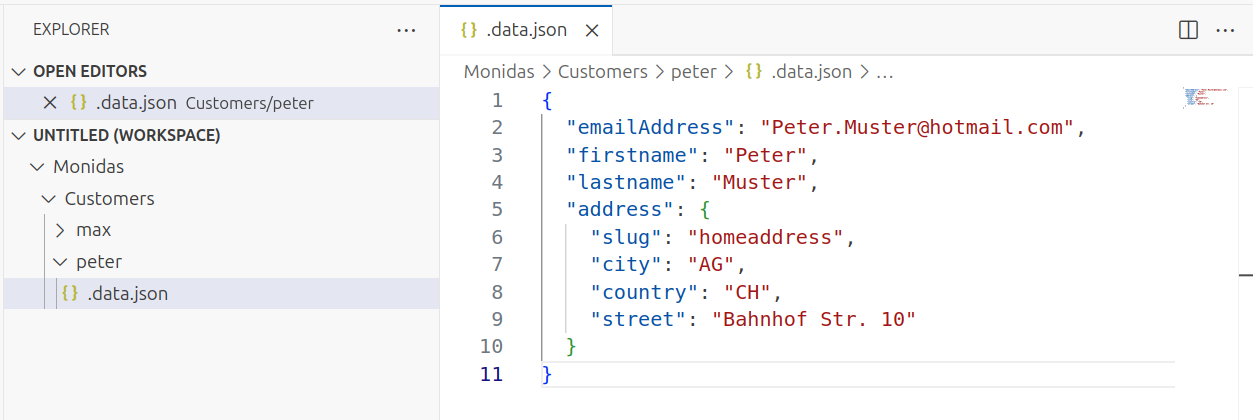
\includegraphics[width=1\linewidth]{inlineEditor.png}
\caption{}
\label{fig:inlineEditor}
\end{figure}

\subsubsection*{Validierung}

\subsubsection*{Abgrenzung}


\subsubsection{Zusammenspiel Explorer und Editor}


\subsection{Umsetzung}
\label{sec:vfs-umsetzung}


\subsubsection{Aufbau des Explorer-Baums}
\label{subsec:explorer-baum}


\subsubsection{Editor-Integration}
\label{subsec:editor-integration}

\subsubsection{Datenvalidierung}
\label{subsec:vfs-validierung}

\subsubsection{Benachrichtigungen und Nutzerfeedback}
\label{subsec:vfs-benachrichtigungen}

\subsection{Bewertung der Lösung}
\label{sec:vfs-bewertung}

%Alle im Explorer dargestellten Ordner sind virtuell und werden erst beim Aufklappen durch den Nutzer geladen („Pull-Prinzip“, siehe Abschnitt~\ref{sec:vfs-konzeption}). Bereits geladene Daten werden temporär im Cache gehalten und erst bei Änderungen, beispielsweise nach einer Umbenennung, erneut abgerufen. Die Datei \texttt{.data.json} enthält beim ersten Anzeigen noch keine Daten. Erst beim Öffnen der Datei im Editor werden die Instanzdaten abgerufen und angezeigt. Eine dauerhafte lokale Speicherung findet nicht statt.
\section{Editorunterstützung }

\subsection{Ziel und Überblick}
Was soll die LSP-Integration leisten? (Navigation, Validierung, Vervollständigung) etc.

\subsection{Problemstellung}
Welche Ansätze gibt es zur Unterstützung im Editor?

\subsection{Umsetzung}

\subsubsection{Validierung}
Welche Felder prüft der LSP? Mit und ohne Constraints. 
Live-Validierung beim Schreiben im Editor.

\subsubsection{Autovervollständigung}
Welche Daten werden angezeigt? Wie werden die Daten geholt – mit und ohne Constraints.

\subsubsection{Go-to-Definition}
Wie funktioniert Go-to-Definition? Momentan über die ID, die im JSON gesetzt ist, usw.
\section{Schlussbemerkungen}


%%---BIBLIOGRAPHY------------------------------------------------------------------------
{\sloppypar
\printbibliography[heading=bibintoc, title=Quellenverzeichnis]
}

%%---APPENDIX----------------------------------------------------------------------------
\section*{Eigenständigkeitserklärung}
\markboth{\MakeUppercase{Eigenständigkeitserklärung}}{\MakeUppercase{Eigenständigkeitserklärung}}

\addcontentsline{toc}{section}{Eigenständigkeitserklärung}

Ich erkläre hiermit, dass ich den vorliegenden Leistungsnachweis selber und selbständig verfasst habe,
\begin{itemize} 
\item dass ich sämtliche nicht von mir selber stammenden Textstellen und anderen Quellen wie Bilder etc. gemäss gängigen wissenschaftlichen Zitierregeln\footnote{IEEE} korrekt zitiert und die verwendeten Quellen klar sichtbar ausgewiesen habe; 
\item dass ich in einer Fussnote oder einem Hilfsmittelverzeichnis alle verwendeten Hilfsmittel (KI-Assistenzsysteme wie Chatbots\footnote{z.B. ChatGPT}, Übersetzungs-\footnote{z.B. Deepl} Paraphrasier-\footnote{z.B. Quillbot} oder Programmierapplikationen\footnote{z.B. Github Copilot}) deklariert und ihre Verwendung bei den entsprechenden Textstellen angegeben habe;
\item dass ich sämtliche immateriellen Rechte an von mir allfällig verwendeten Materialien wie Bilder oder Grafiken erworben habe oder dass diese Materialien von mir selbst erstellt wurde;
\item dass das Thema, die Arbeit oder Teile davon nicht bei einem Leistungsnachweis eines anderen Moduls verwendet wurden, sofern dies nicht ausdrücklich mit der Dozentin oder dem Dozenten im Voraus vereinbart wurde und in der Arbeit ausgewiesen wird; 
\item dass ich mir bewusst bin, dass meine Arbeit auf Plagiate und auf Drittautorschaft menschlichen oder technischen Ursprungs (Künstliche Intelligenz) überprüft werden kann;
\item dass ich mir bewusst bin, dass die Hochschule für Informatik FHNW einen Verstoss gegen diese Eigenständigkeitserklärung bzw. die ihr zugrundeliegenden Studierendenpflichten der Studien- und Prüfungsordnung der Hochschule für Technik verfolgt und dass daraus disziplinarische Folgen (Verweis oder Ausschluss aus dem Studiengang) resultieren können.
\end{itemize}

\vspace*{4ex}

Windisch, 14. August 2025

\vspace*{4ex}

{\renewcommand{\arraystretch}{1.5}
\begin{tabular}{@{}>{\bf}ll}
Name: & Gianni Parrillo\\
Unterschrift: & \\
\end{tabular}
\selectlanguage{ngerman}				%ngerman or english
\begin{appendix} %Anhang
\section{Ein Anhang}

\subsection{Aufgabenstellung im Originalwortlaut}


\subsection{Gesamtübersicht}


\subsection{Berechnungen / Resultate Umfrage}


\subsection{Tests – Screenshots}

\end{appendix}


%%---NOTES for DEBUG---------------------------------------------------------------------
%\newpage
%\listoftodos[\section{Todo-Notes}]
%\clearpage

\end{document}